%%%%%%%%%%%%%%%%%%%%%%%%%%%%%%%%%%%%%%%%%
% Journal Article
% LaTeX Template
% Version 1.3 (9/9/13)
%
% This template has been downloaded from:
% http://www.LaTeXTemplates.com
%
% Original author:
% Frits Wenneker (http://www.howtotex.com)
%
% License:
% CC BY-NC-SA 3.0 (http://creativecommons.org/licenses/by-nc-sa/3.0/)
%
%%%%%%%%%%%%%%%%%%%%%%%%%%%%%%%%%%%%%%%%%
%----------------------------------------------------------------------------------------
%       PACKAGES AND OTHER DOCUMENT CONFIGURATIONS
%----------------------------------------------------------------------------------------
\documentclass[paper=letter, fontsize=10pt]{article}
\usepackage[english]{babel} % English language/hyphenation
\usepackage{amsmath,amsfonts,amsthm} % Math packages
\usepackage[utf8]{inputenc}
\usepackage{blindtext, subcaption, caption, graphicx, float, hyperref, tikz, pgfplots}
% float: Required for tables and figures in the multi-column environment - they need to be placed in specific locations with the [H] (e.g. \begin{table}[H])
% Hyperref: For hyperlinks in the PDF
\usepackage[sc]{mathpazo} % Use the Palatino font
\usepackage[T1]{fontenc} % Use 8-bit encoding that has 256 glyphs
\linespread{1.05} % Line spacing - Palatino needs more space between lines
\usepackage{microtype} % Slightly tweak font spacing for aesthetics
\usepackage[hmarginratio=1:1,top=32mm,columnsep=20pt]{geometry} % Document margins
\usepackage{multicol} % Used for the two-column layout of the document
%\usepackage[hang, small,labelfont=bf,up,textfont=it,up]{caption} % Custom captions under/above floats in tables or figures
\usepackage{booktabs} % Horizontal rules in tables
\usepackage{lettrine} % The lettrine is the first enlarged letter at the beginning of the text
\usepackage{paralist} % Used for the compactitem environment which makes bullet points with less space between them
\usepackage{abstract} % Allows abstract customization
\renewcommand{\abstractnamefont}{\normalfont\bfseries} % Set the "Abstract" text to bold
\renewcommand{\abstracttextfont}{\normalfont\small\itshape} % Set the abstract itself to small italic text
\usepackage{titlesec} % Allows customization of titles
\usepackage{soul} % Provides the ability to cross-out text
\usepackage{listings} % Code snippets and syntax highlight
\usepackage{fontspec}
\usepackage{minted}

\renewcommand\thesection{\Roman{section}} % Roman numerals for the sections
\renewcommand\thesubsection{\Roman{subsection}} % Roman numerals for subsections

\titleformat{\section}[block]{\large\scshape\centering}{\thesection.}{1em}{} % Change the look of the section titles
\titleformat{\subsection}[block]{\large}{\thesubsection.}{1em}{} % Change the look of the section titles
\newcommand{\horrule}[1]{\rule{\linewidth}{#1}} % Create horizontal rule command with 1 argument of height
\usepackage{fancyhdr} % Headers and footers
\pagestyle{fancy} % All pages have headers and footers
\fancyhead{} % Blank out the default header
\fancyfoot{} % Blank out the default footer

\fancyhead[C]{University of Southern Denmark $\bullet$ RM-UAST $\bullet$ Spring 2017 $\bullet$ Group 5 } % Custom header text

\fancyfoot[RO,LE]{\thepage} % Custom footer text
%----------------------------------------------------------------------------------------
%       TITLE SECTION
%----------------------------------------------------------------------------------------
\title{\vspace{-15mm}\fontsize{24pt}{10pt}\selectfont\textbf{Module Seven }} % Article title
\author{
\large
{\textsc{}}\\[2mm]
{\textsc{Henrik Frank, hefra13@student.sdu.dk }}\\[2mm]
{\textsc{Christian Arentsen, chare13@student.sdu.dk }}\\[2mm]
{\textsc{Vasileios Karvouniaris, vakar15@student.sdu.dk }}\\[2mm]
{\textsc{Asbjørn Schou Müller, asmul10@student.sdu.dk }}
%\thanks{A thank you or further information}\\ % Your name
%\normalsize \href{mailto:marco.torres.810@gmail.com}{marco.torres.810@gmail.com}\\[2mm] % Your email address
}
\date{}

%----------------------------------------------------------------------------------------
\begin{document}
\maketitle % Insert title
\thispagestyle{fancy} % All pages have headers and footers


\section{AQ Ground Control}
\subsection{Inspecting AutoQuad log files}
\paragraph{UKF\_POSD}
For the down position, as seen i Figure~\ref{ukf_down} it can be seen that the positions are actually positive, though it should be negative values, as we are measuring going down as positive. Regardless, we can see, after the GPS has gotten a fixed position, we get an altitude of approx 10 meters above sea level, and we can see how the drone takes off, and lands again a couple of times. 
\begin{figure}
\centering
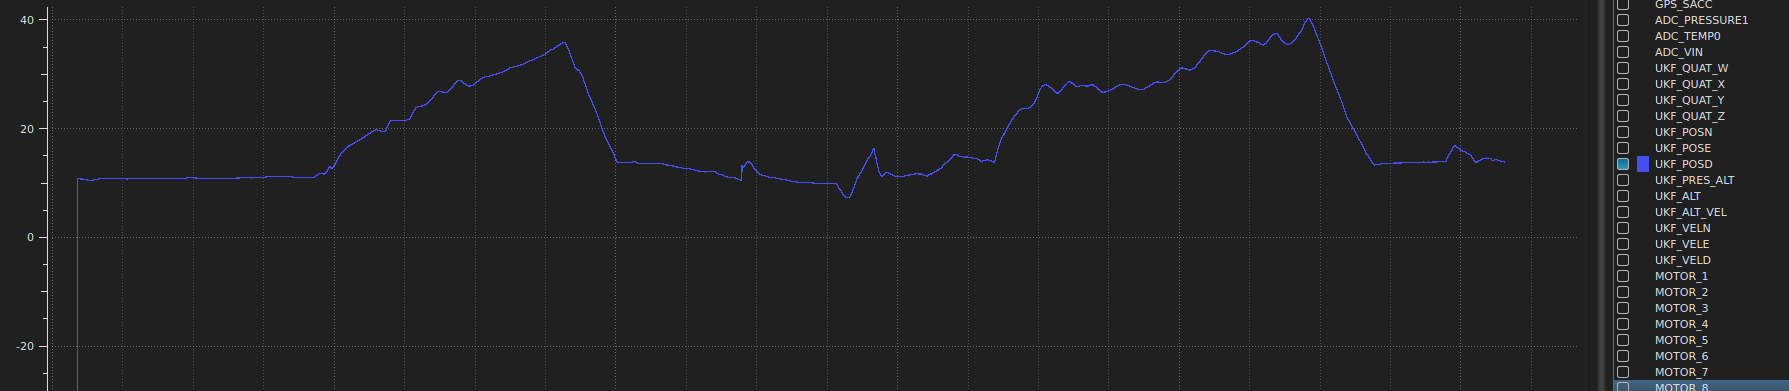
\includegraphics[width=1\textwidth]{Figures/UKF_POSD}
\caption{Graph showing UKF\_POSD for down}
\label{ukf_down}
\end{figure}


\paragraph{UKF\_POSN, UKF\_POSE and UKF\_POSD}
For all positions in the coordinate system, Figure~\ref{ukf_all}, it can be seen how the drone moves around.

\begin{figure}
\centering
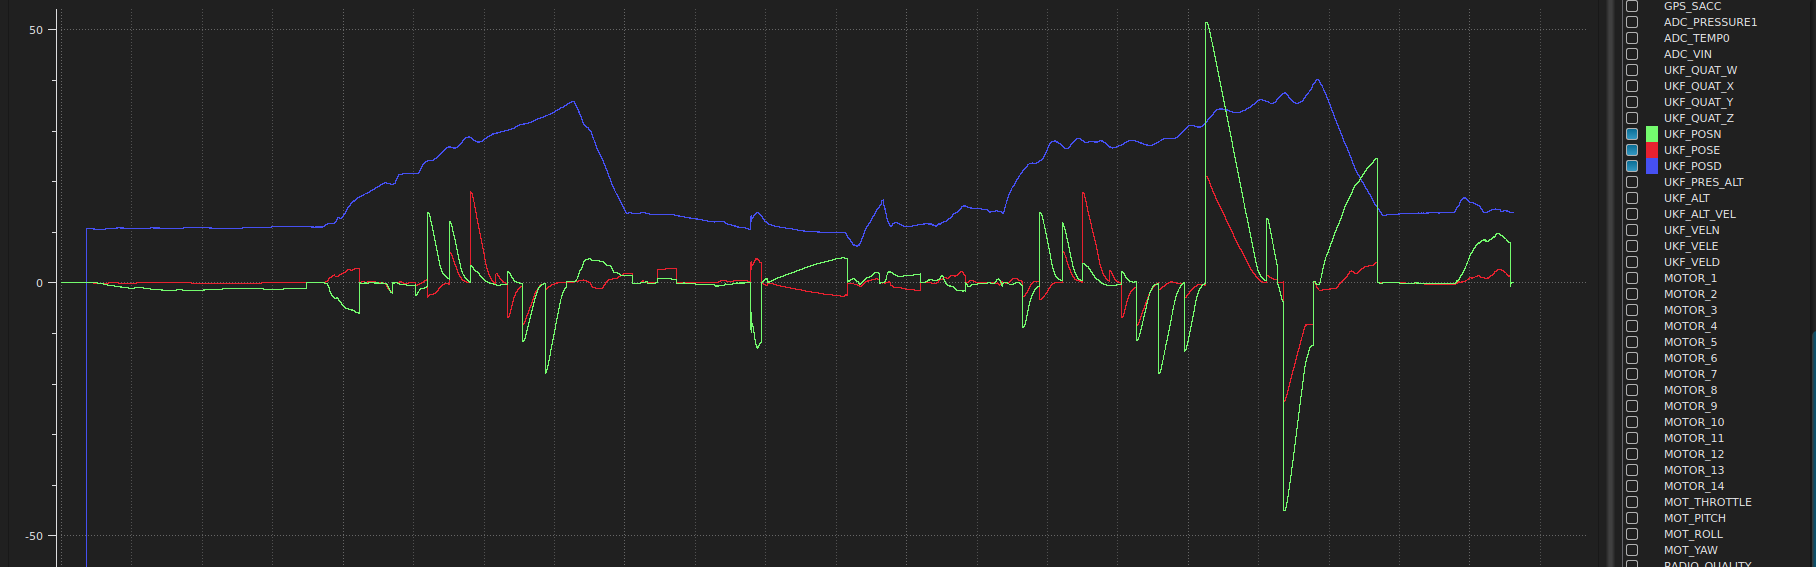
\includegraphics[width=1\textwidth]{Figures/UKF_All}
\caption{Graph showing UKF coordinates for North, East and Down}
\label{ukf_all}
\end{figure}

\subsubsection{Generating mission route plans}
Use the \texttt{aqlogreader} Python script available in the module folder to import track data from the file \texttt{021-AQL.LOG}. 
\paragraph{}
Create a Python class to generate a route plan consisting of waypoints (latitude, longitude, altitude, heading) based on the track data removing excessive track points.

The class should perform the conversion base on the different input parameters below: 
\begin{enumerate}
\item maximum distance deviation from track (multirotor).
\item \st{maximum waypoints allowed (multirotor).}
\item \st{maximum distance and bearing angle deviation from track (fixed wing).}
\end{enumerate}

\paragraph{}
Please look into the literature to find existing algorithms or devise your own.
Plot both the track log and generated route plan using Google Earth using the \texttt{export\_kml.py} class available under course materials.
Test your route plan class using as input the NMEA data (for which you developed an import class in module 1) from the file \texttt{nmea\_trimble\_gnss\_eduquad\_flight.txt}

Present the algorithm, your results and discuss advantages/disadvantages in the report.
\paragraph{Results}


In order to remove excessive points from the track we estimated the Euclidean distance from one point to consecutive points. Then we set as a checkpoint the one whose distance from the 'point of origin' was larger than a threshold. And we repeat the process each time with the new checkpoint as the point of origin for the following points.

\begin{minted}[mathescape,
%                linenos,
               numbersep=5pt,
               gobble=2,
               frame=lines,
               framesep=2mm]{python}
   from math import hypot
        ...
        dstnc = hypot(nextLat, nextLng)
        dstnc = hypot(dstnc, nextAlt)
        if dstnc >= threshold:
            initLat = oldLat
            initLng = oldLng
            initAlt = coords
            cpLat.append(oldLat)
            cpLng.append(oldLng)
            corAlt.append(coords)
        ...
\end{minted}
By applying this method on the data in \textit{021-AQL.LOG} file we managed to get a good fit from the original points with threshold=1 (Figure \ref{fig:thresh1}). The amount of checkpoints in this case was 382. Then we increased the threshold to 5 and the points dropped to 76! the fit however was less than optimal (Figure \ref{fig:thresh5}). The process was also applied on the Nmea data from \textit{nmea\_trimble\_gnss\_eduquad\_flight.txt} with produced an impressive amount of 157 points out of the original 5500+ points (Figure \ref{fig:Nmea.3}).


\begin{figure}
\centering
\begin{minipage}{.5\textwidth}
	\centering
	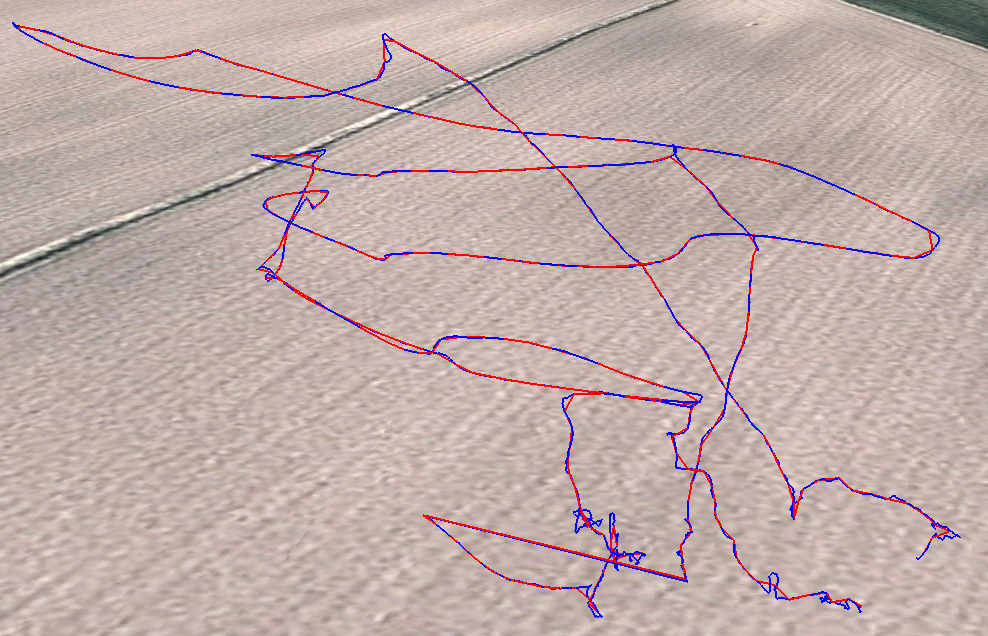
\includegraphics[width=.8\linewidth]{Figures/Paths_threshold_1_w_alt}
	\caption{\textit{Threshold 1}}
	\label{fig:thresh1}
\end{minipage}%
\begin{minipage}{.5\textwidth}
	\centering
	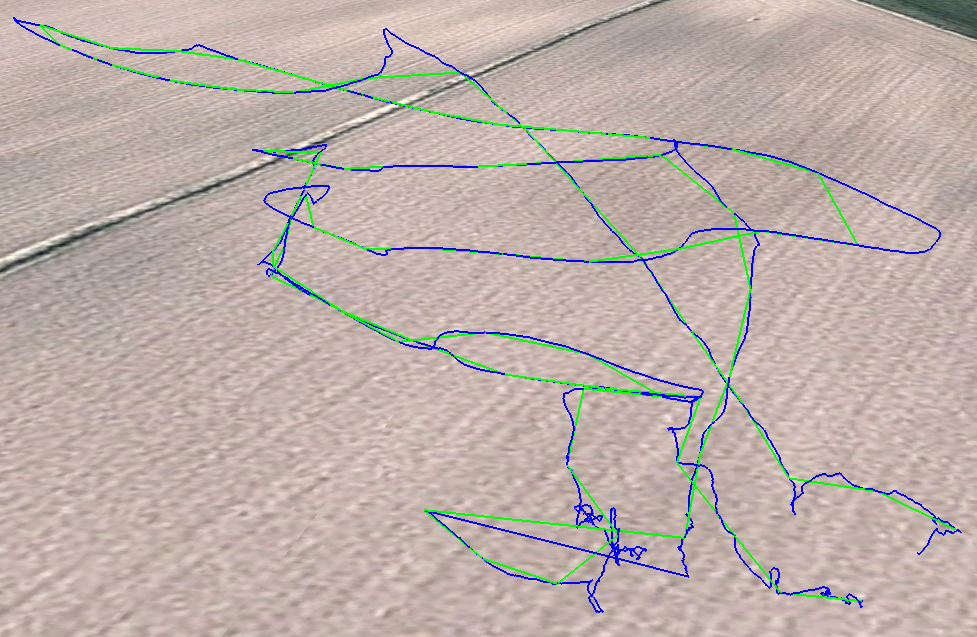
\includegraphics[width=.8\linewidth]{Figures/Paths_threshold_5_w_alt}
	\caption{\textit{Threshold 5}}
	\label{fig:thresh5}
\end{minipage}
\end{figure}

\begin{figure}
\centering
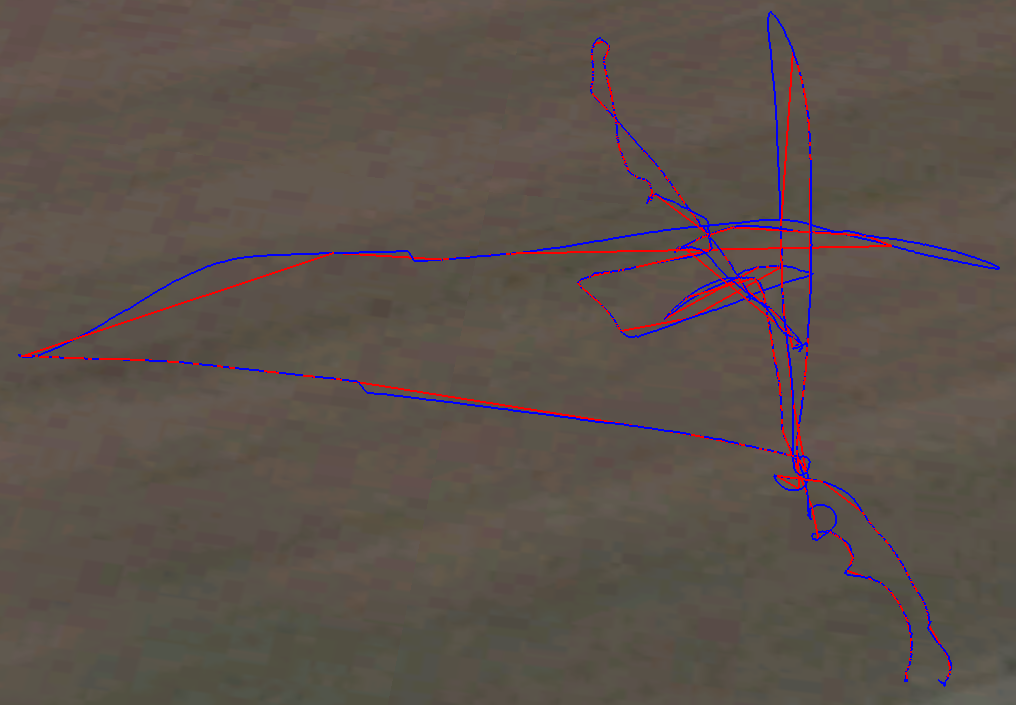
\includegraphics[width=.5\textwidth]{Figures/Nmea_threshold_0_3_w_alt}
\caption{Nmea Data with Threshold 0.3}
\label{fig:Nmea.3}
\end{figure}


The main advantage of this approach is its simplicity. It is very easy to implement and seems rather intuitive. On the other hand it lacks consistent performance across different kinds of data. For example a threshold of 0.3 is needed for the Nmea data to get a total of 157 out of 5531 points while a threshold of 1 is sufficient for 382 out of 2500 points in the AQL data.
%\pagebreak
%¤
%\bibliographystyle{plain}
%https://en.wikipedia.org/wiki/Line-of-sight_propagation
%\bibliography{bibfile}
%----------------------------------------------------------------------------------------
%\end{multicols}
\end{document}
